\subsubsection{Player Unit Tests}
The structure of units tests for the different grains are largely the same, except maybe for player. If we look at \autoref{BuildRep} and \autoref{BuildPlayer} \todo{Same here}, we discussed the idea of dead code and modularization. In short, because of the high coupling between the grains, decomposition proved to be more difficult as we had not taken the high coupling into account earlier in the process. However, with tests it was both simpler per default and we had a focus on making it simple to decompose. \\
\begin{figure}[h]
    \centering
    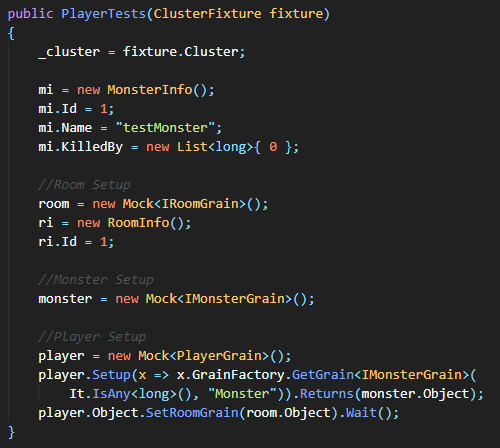
\includegraphics[width=0.7\linewidth]{Materials/TestingDiscussion/PlayerTestConstructor}
    \caption{The constructor for the player tests, showcasing how we chose to include the essentials for initialization.}
    \label{PlayerTestConstructor}
\end{figure}
If we look at \autoref{PlayerTestConstructor} we can see how we chose to setup the player tests. This setup is independent of the variation of the game we choose. Since we also have tests that are independent of variations, meaning they are included across all variations, the room mock and monster mock are initialized in the constructor. So, in tests that include the boss we chose to create the boss mock inside of those tests instead of in the setup alongside room and monster. There are two reasons for this. First off, as player does not include many boss tests we deemed it unnecessary to include in general setup. The second reason was to keep decomposition as simple as possible. If we keep the things affected by variations inside test cases we can decompose and combinate on a function level. This means, unlike in the grain decomposition, we do not have to insert lines of code here and there. This also means that the variations of abilities the player can take, fireball, roar and none, are not intersected in each others test \todo{Not exactly sure what you mean? Don't we use ability to intersect?}. That is, for instance, fireball is not tested inside a damage test but these damage tests are kept separate. So, with this in mind, we can look at the CLS part of the tests and how we combinate those. \\
\\
Since tests of course are dependent on the grains, we can reuse some of the semantics from the grains. If we compare \autoref{semanticPlayerTest} to \autoref{SemanticTargetPlayer} from \autoref{BuildPlayer}, we can see that they are both alike, where our semanticPlayerTestTargets differ in having another semantic type input in \textit{'playerTest} \todo{After a couple of re-reads I think I understand what you are saying, but could be more clear, especially when saying they are alike and differ at the same timer}. 
\begin{figure}[h]
    \centering
    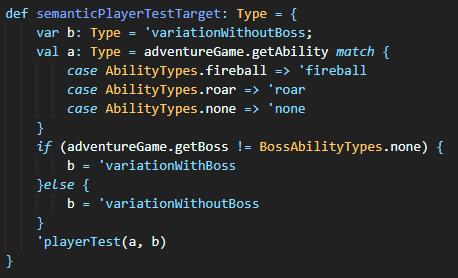
\includegraphics[width=0.7\linewidth]{Materials/TestingDiscussion/SemanticPlayerTestTarget}
    \caption{The function determining the semantic types for player tests.}
    \label{semanticPlayerTest}
\end{figure}
The reason we have the boss included in the semantic target is due to the fact that our player tests can be split in five parts. The first part \todo{What is the first part?} of \autoref{semanticPlayerTest} would suffice for the first three parts of the player tests, which are the essential tests that will be included in all variations, the tests specific for roar and the tests specific for fireball. Then we have a test dealing damage to the boss. Most notably, one of our testcases include casting a fireball on the boss. That specific test is both dependent on a boss being present in the game variation and that the player ability is of type fireball. Only when those two criteria are fulfilled can we include that test. So with variations that vary both on the player's abilities and the presence of the boss, how did we combinate this? \\
Semantically, we have split these combinators into three parts: \textit{'boss}, which contains the tests that are only dependent on the boss being a part of the game. That is, these tests do not use the player's abilities, but only the boss. The next semantic type is \textit{'bossPresent}. These combinators include tests that rely both on the player's ability and the boss. However, since we only have a single case where these overlap, it is only the \textit{'bossPresent('fireball, 'variationWithBoss)} that actually inserts a test, as there are no tests of roar and boss. The last semantic type is \textit{'testAbility} which contains the tests that are only specific for the player's ability. With these three parts, we can succesfully combinate all the possible variations of player tests that vary depending on ability and boss presence. Because of this, we can then describe player tests as: \textit{string $\cap$ boss, string $\cap$ bossPresent, string $\cap$ testAbility $\to$ MyResult $\cap$ playerTest}\todo{forklar bedre? Er det korrekt? Nej, ikke helt så simpelt} \todo{Ved ikke hvad indforstået hedder på engelsk, men et meget indforstået afsnit som ville have stor gavn af en eller anden form for diagram til at vise hvad du mener. Måske noget lignende en taxonomy ligesom i CLS afsnittet?}. \\
\\
This structure of the combinators is only due to the fireball boss test, which means that this intermediate step with the type of \textit{'bossPresent} is only truly meaningful when it comes to the fireball and boss variation. Because of this way we did the player tests, there are somewhat empty intermediate combinators for the abilities roar and none. That is, no tests are to be implemented that relies on the roar ability and the presence of the boss. We could argue that this opens up for the possibility of changing roar in a way that affects the boss, such that we needed tests that are dependent on these two. If this was the case, these new tests could easily be inserted into the intermediate combinator. However, we will not and do not expect roar to change in such a way to affect the boss directly, given the nature of the ability. This means that this structure of the player test combinators may seem somewhat redundant, due to the fact that the intermediate step, that is the intermediate combinators, is only needed for one specific case. So, if we were to look at the combinators of roar isolated, the intermediate step may seem irrelevant or puzzling. \todo{I dunno, kringlet? finno? Lyder fint}